\chapter{Results}\label{ch:results}

\section{DSN System Requirements}\label{sec:dsn-system-requirements}

In the Evaluation chapter I examined the theoretical bounds of DSN system requirements both with TTL (Section~\ref{sssec:evaluation_of_ttl}) and without TTL (Section~\ref{sssec:eval_of_dsn_system_requirements}) for the OPQ and Lokahi networks.

This section will focus on examining the actual DSN system requirements for the OPQ and Lokahi networks.

All results in this section were gathered directly from the OPQ and Lokahi networks and no estimated parameters or simulations were used.

\subsection{DSN System Requirements: OPQ}\label{subsec:dsn-system-requirements:-opq}

System utilization metrics were collected during the deployment of the OPQ DSN. The metrics that were collected are provided in the description of the SystemStatsPlugin (Section~\ref{lbl:SystemStatsPlugin}). In summary, I collected metrics on plugin utilization, system resource utilization, garbage collection, tunable Laha parameters, and storage requirements for each level within the Laha hierarchy.

There were several schema changes to the stored metric data, with the most significant change taking place on September 20, 2019. For these results, I only used metrics collected after this date as they contain the most useful data.

Further, the astute reader will notice that there are often times more than 15 Boxes in the metric data when only 15 Boxes were deployed for the UHM deployment. This is attributed to the fact that several Boxes were sent to the Electric Power Research Institute (EPRI) to evaluate if our Boxes could be used as a test bed for their power quality analysis needs. The metrics collected by Laha are collected for the total set of all Boxes sending to OPQ, and thus, also sometimes include metrics from the Boxes that EPRI are evaluating.

First I will examine the storage requirements at each level within the hierarchy. Then I will compare the levels to each other to get an idea of the requirements for the entire network. Finally, I will compare these values to the theoretical bounds found in previous sections.

\subsubsection{DSN System Requirements OPQ: IML}

The Instantaneous Measurements Level (IML) contains a window of raw samples from sensors. In the case OPQ, these consist of the samples of data stored in the main memory of each OPQ Box. The IML has a TTL of 15 minutes which is determined by the available storage capacity of each OPQ Box.

The IML is unique in that data from the IML is never ``saved" by higher levels in the hierarchy. Instead, IML data is copied into Detections, Incidents, and Phenomena. Because of this, the size of the IML over time is function of the number of OPQ Boxes sending data at any particular time. Figure~\ref{fig:actual_iml_opq} shows the actual OPQ IML data growth over the deployment period. As can be observed, the AML size is a simple function of the number of OPQ Boxes sending data.

\begin{figure}[H]
    \centering
    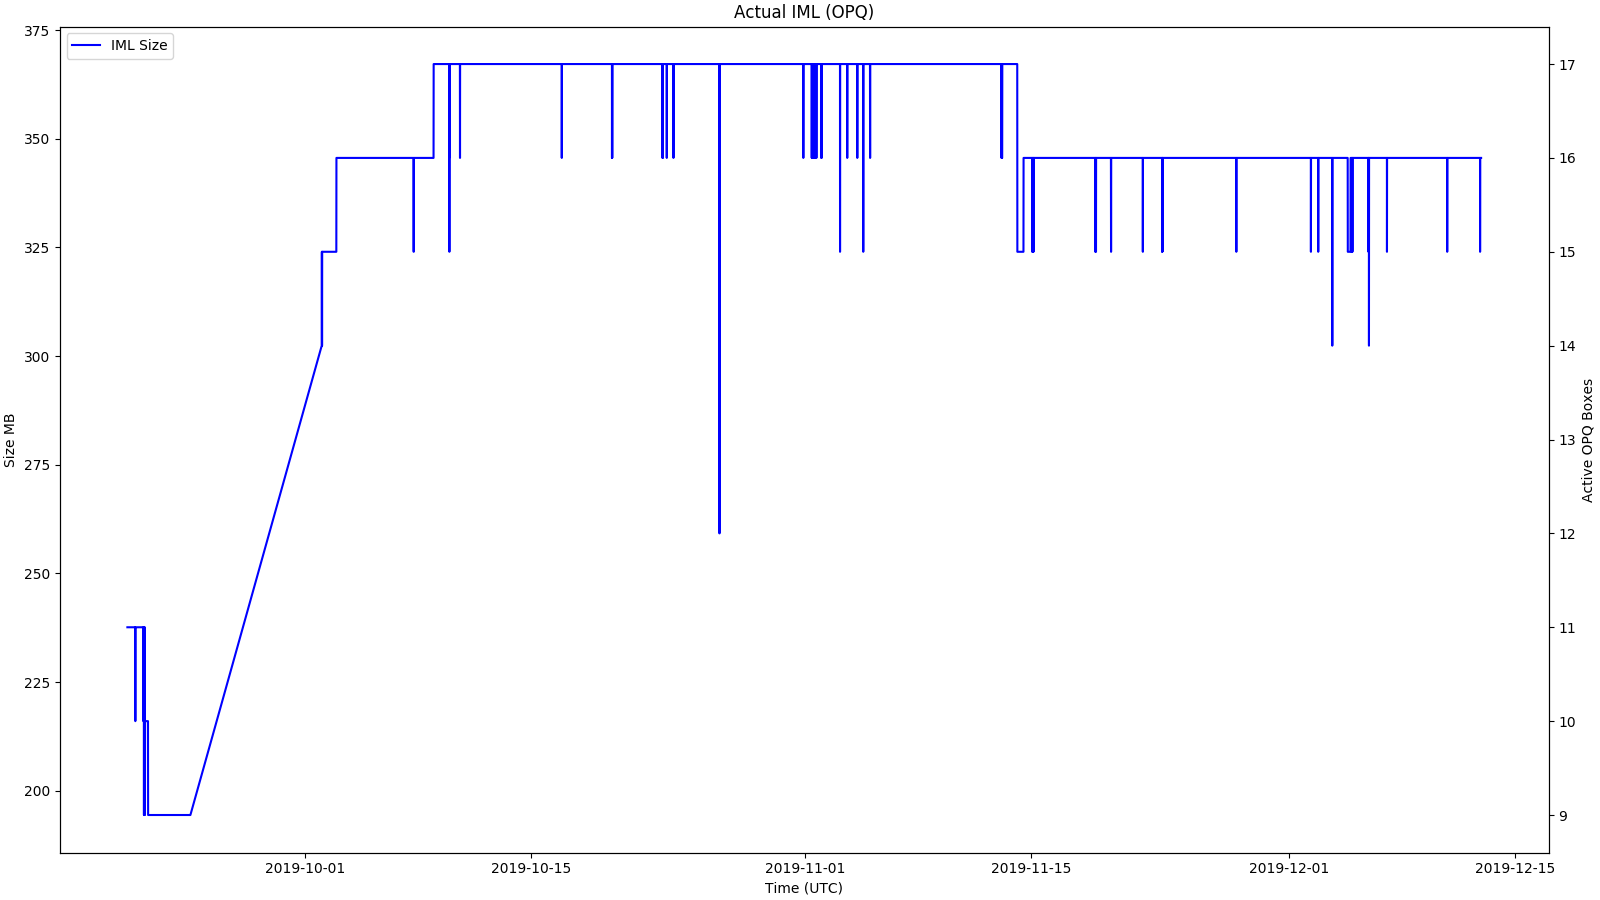
\includegraphics[width=\linewidth]{figures/actual_iml_opq.png}
    \caption{Actual IML for OPQ}
    \label{fig:actual_iml_opq}
\end{figure}

A deployment of 15 OPQ Boxes will consume about 325 MB of IML space.

\subsubsection{DSN System Requirements OPQ: AML}

The Aggregate Measurements Level (AML) contains summary statistics of features extracted from the IML. OPQ contains two sub-levels within the AML (Measurements and Trends). Data within the AML can be saved by higher levels within Laha (DL, IL, and PL). If AML data is saved, it receives the TTL of the highest level that the data was saved by.

I examine the AML data growth for OPQ by looking at the data growth of Measurements, Trends, and the total AML. Figure~\ref{fig:actual_aml_opq} displays the AML growth for the OPQ network as well as statistics about garbage collection.

\begin{figure}[H]
    \centering
    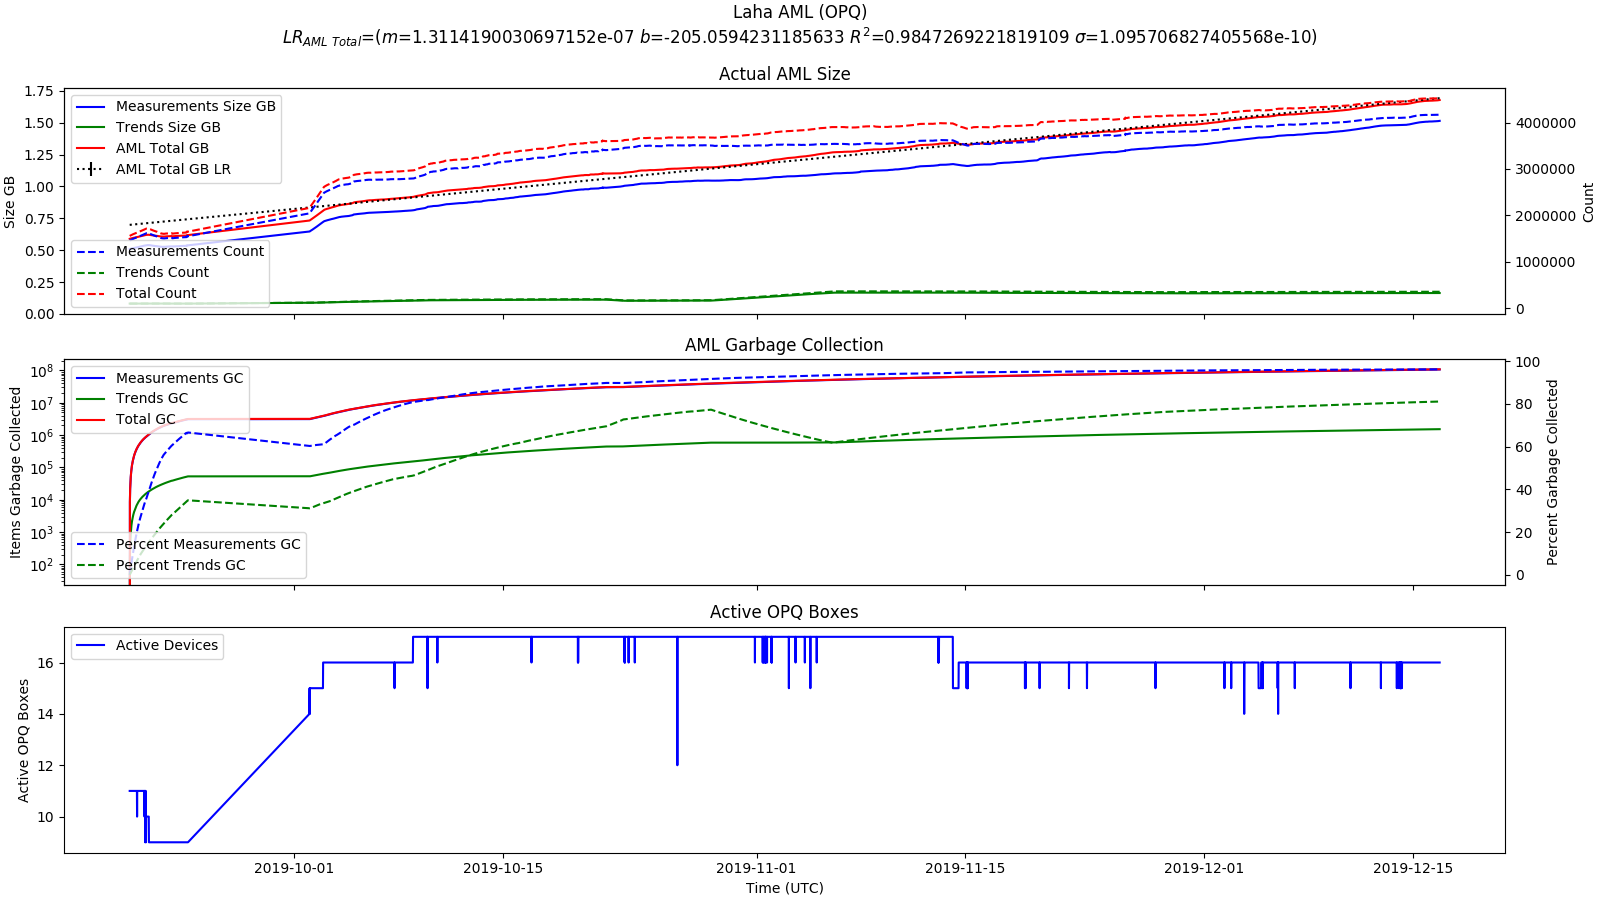
\includegraphics[width=\linewidth]{figures/actual_aml_opq.png}
    \caption{Actual AML for OPQ}
    \label{fig:actual_aml_opq}
\end{figure}

The top panel displays the AML data growth with size in GB on the left Y-axis and the count of AML items on the right Y-axis. Over a period of two and a half months the AML in OPQ has reached a size of about 1.75 GB containing over 4 million AML items.

The middle panel displays the number of Measurements and Trends that were garbage collected over time on the left Y-axis and the percentage of items that were garbage collected on the right Y-axis. About 98\% of all AML data was garbage collected. About 2\% of all AML data is either awaiting garbage collection of was ``saved" by a higher level in the Laha hierarchy.

The bottom panel displays the number of active OPQ Boxes over time. It's possible to see how the number of Boxes impacts the size of the AML. For example, the increase in Boxes in September and the decrease of Boxes in mid-November have noticeable impacts on the AML storage size.

\subsubsection{DSN System Requirements OPQ: DL}

The Detections Level (DL) contains metadata and data bounded by a time window that may or may not contain signals of interest. Detections are generated by threshold based triggering algorithms. Detections can be saved by higher levels in the Laha hierarchy (IL and PL) and will receive the same TTL as the highest level the DL data is saved by. The DL contains metadata about the window it examines, but the bulk of data is produced by the raw samples that get copied into the DL when a Detection is created.

Figure~\ref{fig:actual_dl_opq} shows the DL data growth for the OPQ network over time.

\begin{figure}[H]
    \centering
    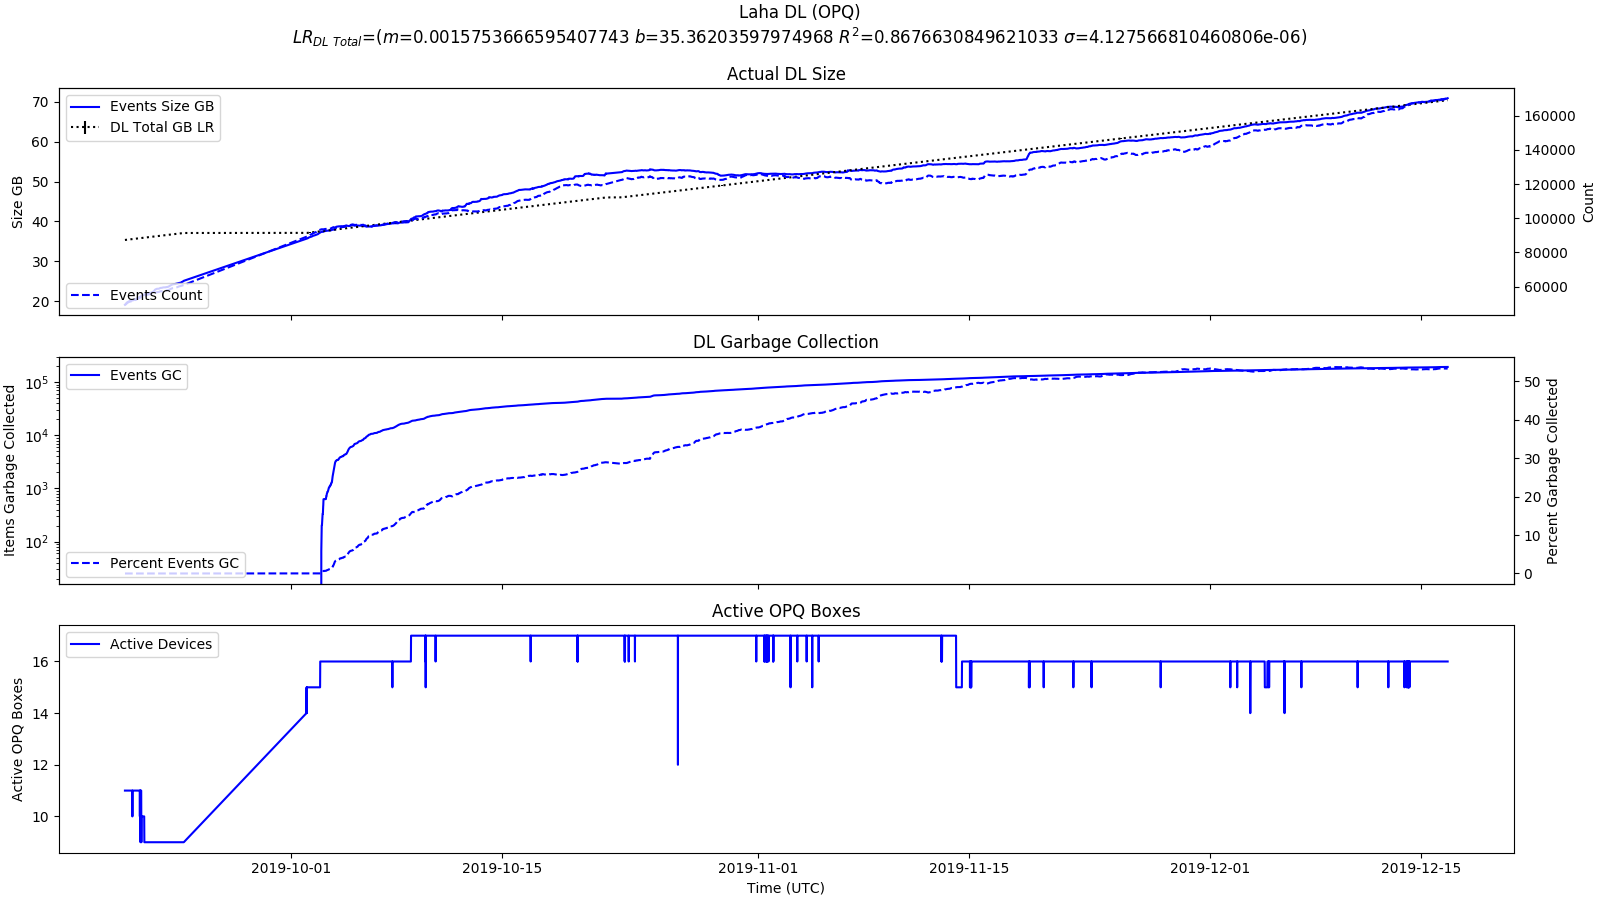
\includegraphics[width=\linewidth]{figures/actual_dl_opq.png}
    \caption{Actual DL for OPQ}
    \label{fig:actual_dl_opq}
\end{figure}

The top panel shows the size of the DL over time with the size in GB on the left Y-axis and the count of Detections on the right Y-axis. The size of the DL for the OPQ network has grown to close 70 GB over the period of two and half months containing a total of 160,000 Detections.

The middle panel shows the garbage collection statistics for the DL. Of note is the delayed uptick in garbage collection until October 1, 2019. This is a direct result of the fact that Detections have a TTL of 1 month, and thus, no Detections were garbage collected during the first month of data collection. As of two and a half months of data collection, about 50\% of all Detections generated have been garbage collected while the other 50\% are wither awaiting garbage collection or have been saved by Incidents or Phenomena.

The bottom panel shows the number of active OPQ Boxes sending data over time.

\subsubsection{DSN System Requirements OPQ: IL}

The Incidents Level (IL) contains metadata and data relating to classified signals of interest. Incidents are created when a Mauka plugin classifies a signal of interest from a Detection. Incidents can be saved by Phenomena.

Figure~\ref{fig:actual_il_opq} shows the IL growth for the OPQ network over a period of two and a half months.

\begin{figure}[H]
    \centering
    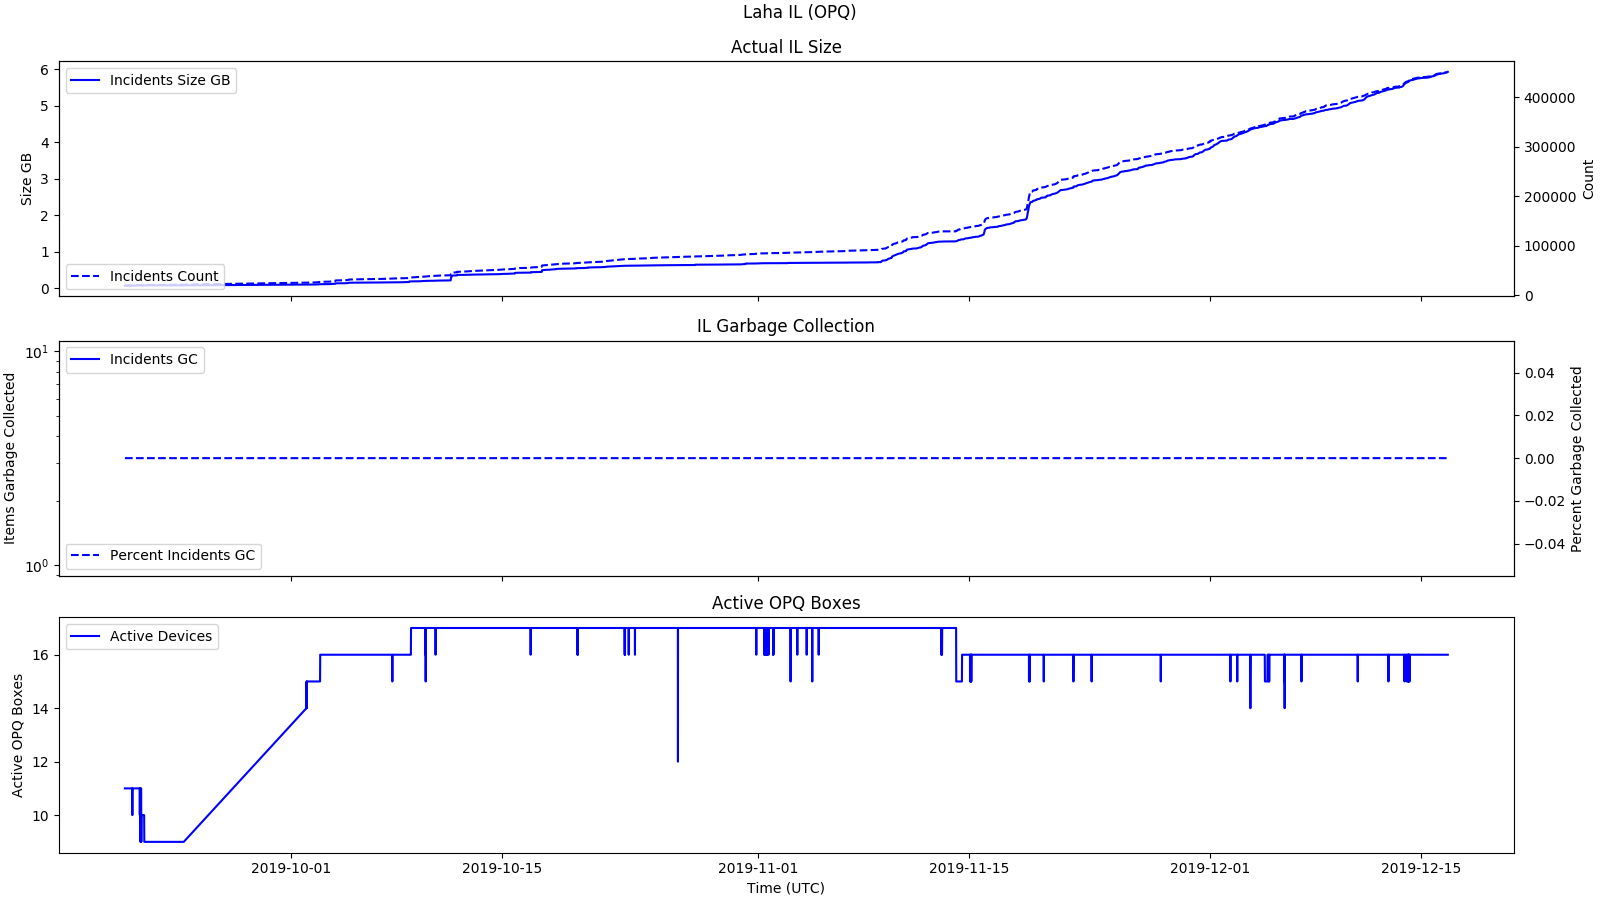
\includegraphics[width=\linewidth]{figures/actual_il_opq.png}
    \caption{Actual IL for OPQ}
    \label{fig:actual_il_opq}
\end{figure}

The top panel shows the growth of the IL with the size in GB on the left Y-axis and the number of Incidents on the right Y-axis. Over a period of two and a half months, the IL of OPQ has grown to near 6GB containing over 400,000 Incidents.

The middle panel shows the garbage collection statistics for the IL. You'll note that the GC statistics are flat lining at 0. This is due to the fact that Incidents are given a default TTL of 1 year and this deployment has only been collecting data for 3 months.

The bottom panel shows the number of active OPQ Boxes sending data over time.

\subsubsection{DSN System Requirements OPQ: PL}

% TODO
TODO

\subsubsection{DSN System Requirements OPQ}

I will now examine the results of combining all Laha levels within OPQ. Figure~\ref{fig:actual_laha_opq} provides the results of data collection for the entire OPQ network over a period of 2 and a half months.

\begin{figure}[H]
    \centering
    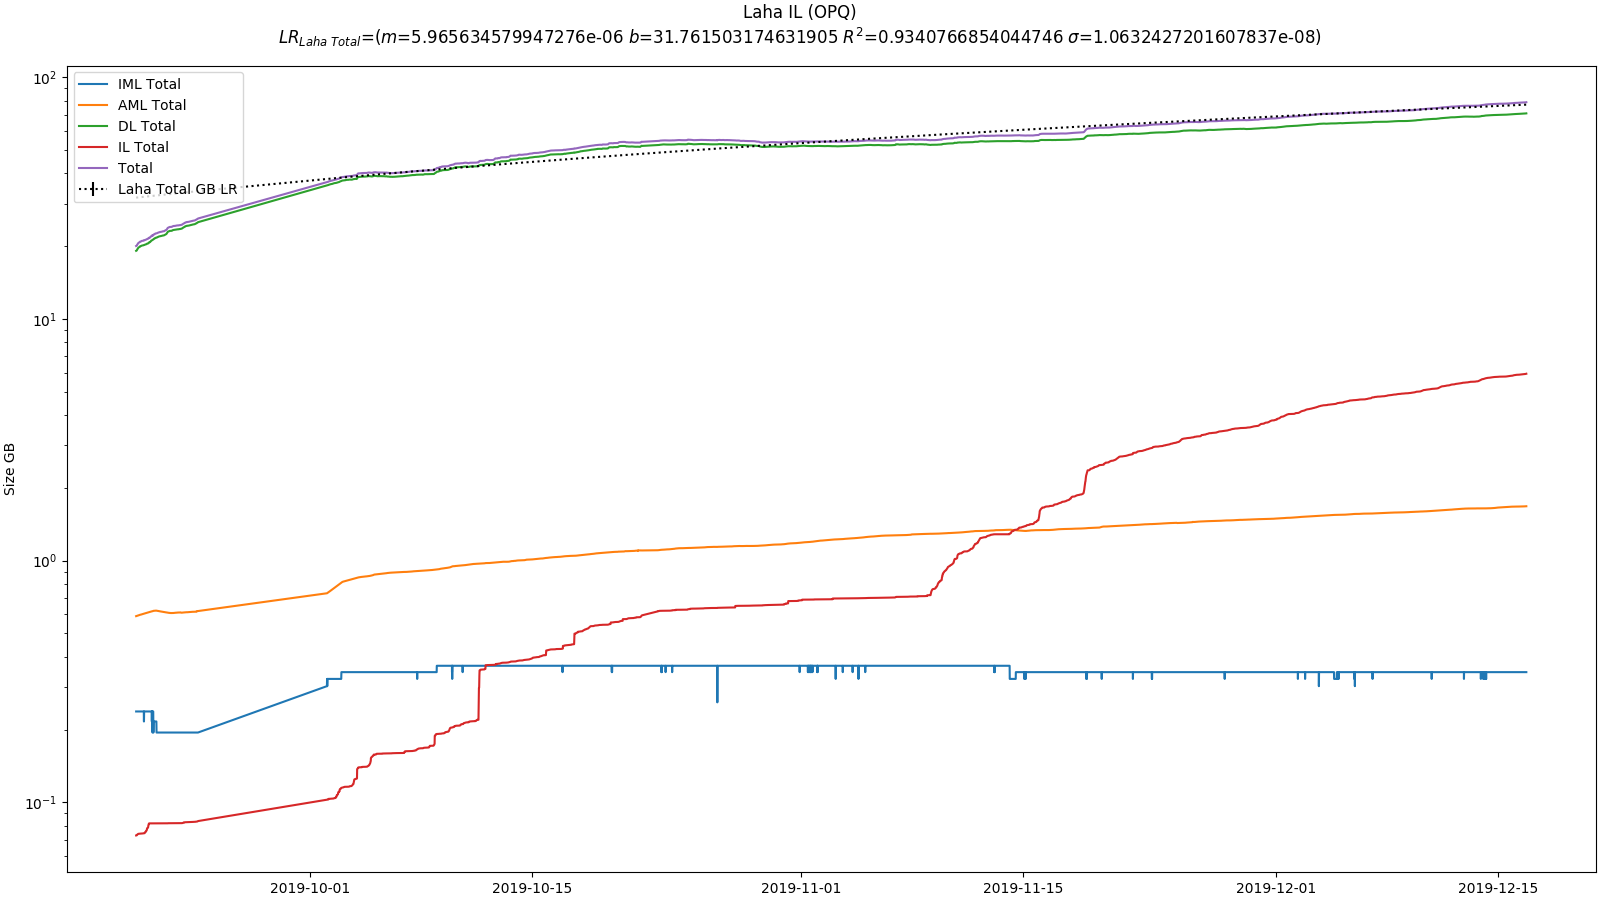
\includegraphics[width=\linewidth]{figures/actual_laha_opq.png}
    \caption{Actual Laha for OPQ}
    \label{fig:actual_laha_opq}
\end{figure}

First, please note that the Y-axis is using a log scale in order to better display the data growth of some of the smaller Laha levels. Next, we observe that the size of the entire network is just under 100 GB over a period of two and a half months with an average of 15 OPQ Boxes.

We can observe that the IML level converges to the smallest of the levels due to its strict 15 minute TTL.

The IL starts out small, but as Incidents are identified, the IL surpasses the IML at about 1 month and surpasses the AML in size at about 2 months. The Detections level is the largest and this makes sense since we treat Detections relatively cheaply and they contain windows of data that are generally larger than the signal of interest if there even is a signal of interest at all.

\subsubsection{DSN System Requirements OPQ: Comparing Results to Estimates}

Now that I have shown the results for the actual DSN storage requirements, I will next compare these results to the estimated storage requirements with and without TTL\@.

Let us first compare the results to the estimated storage requirements without TTL found in Section~\ref{sssec:eval_of_dsn_system_requirements}. This might feel a bit contrived, but the purpose of these results is to show how OPQ compares to a similar system that would collect everything.

One interesting thing to note is that I expected the estimated values to be much higher than the actual values due to the fact that I was not including TTL explicitly anywhere in the estimations. It turns out this is not always the case. The reason for this is that the estimated values are computed by multiplying the amount of time the system has been running with the data rate obtained from the OPQ database for Events, Incidents, and Phenomena, and on the surface, it does not appear that TTL is being used in these estimations. However, this is not exactly the case. The data rate parameters obtained from the OPQ database implicitly have the TTL built in. That is because I measure the data rate over all available Events, Incidents, and Phenomena, but this data rate does not include Incidents, Events, or Phenomena that have been garbage collected! Unfortunately, I do not have detailed metrics on data that was garbage collected (only counts). Any future DSN utilizing Laha should consider recording detailed metrics about data that was garbage collected (duration, data stored, etc).

This really only affects Detections, Incidents, and Phenomena which use estimated database parameters. Samples, Measurements, and Trends are not affected because they are computed directly from the time length without using any estimated database parameters.

The end result of this is that it turns out that the method I use to estimate Events, Incidents, and Phenomena without TTL pretty accurately portray the size of the actual data with TTL.

There was already data in the database before we started collected enhanced metrics. This is true for the AML, DL, IL, and PL. In order to accurately compare data growths from zero, the first value at each level is subtracted from the entire data set at each level. This essentially ``forces" the data set to start at 0 so that we can compare it directly to the estimates.

\paragraph{IML Versus Estimated Growth}
The Instantaneous Measurements Level (IML) consists of raw samples from sensors. Figure~\ref{fig:actual_iml_vs_unbounded_opq} shows the actual IML vs unbounded IML\@.

\begin{figure}[H]
    \centering
    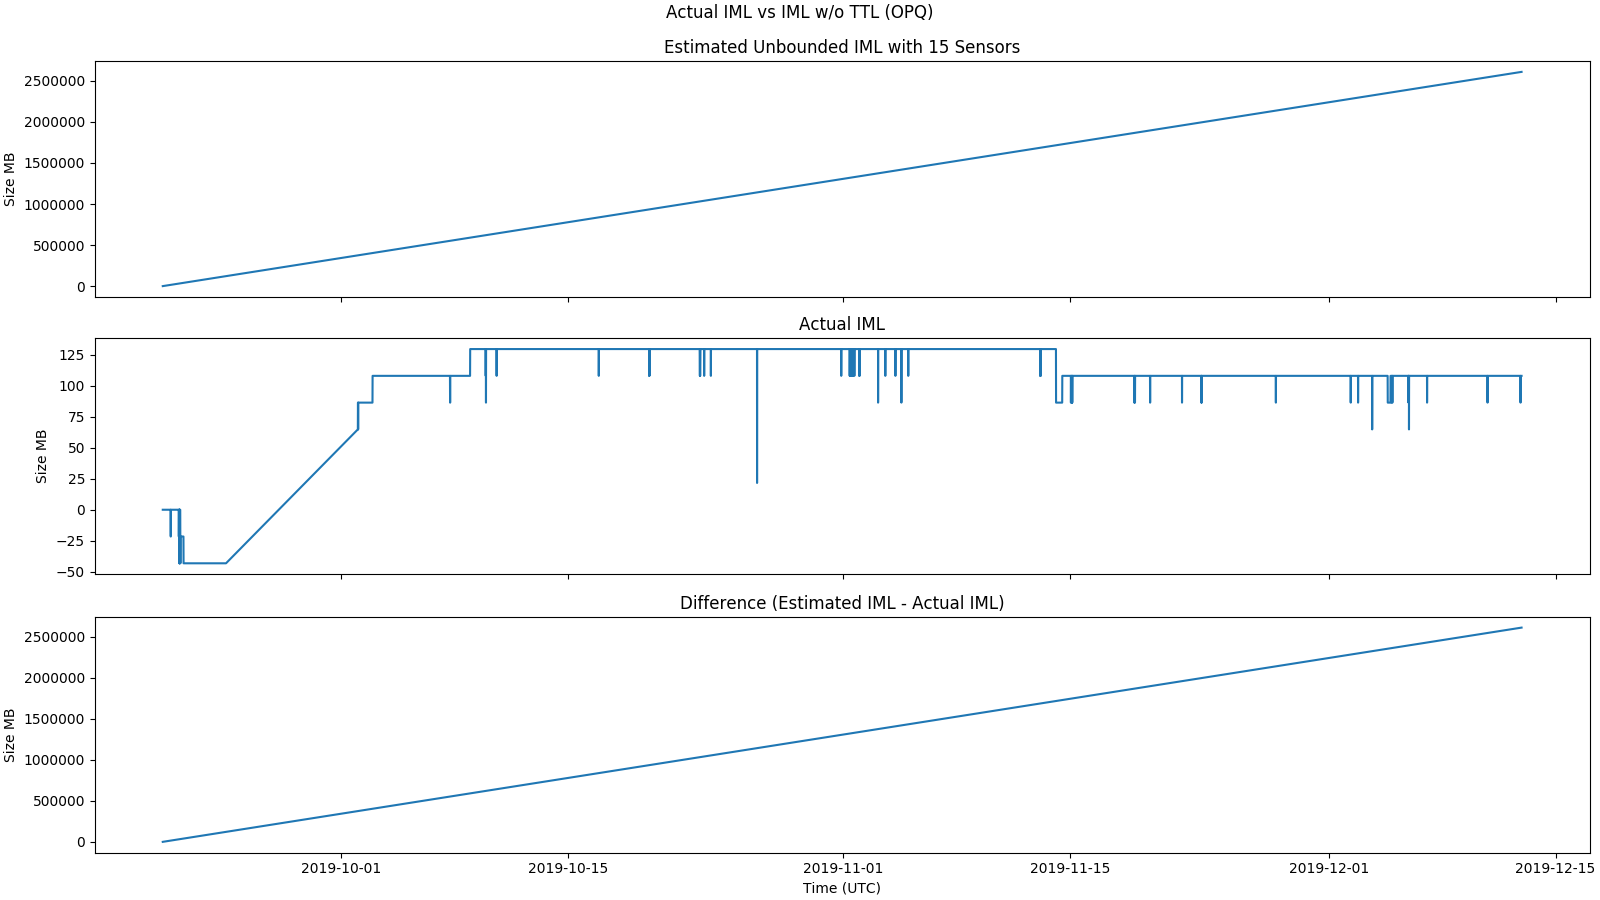
\includegraphics[width=\linewidth]{figures/actual_iml_vs_unbounded_opq.png}
    \caption{Actual IML vs Unbounded IML for OPQ}
    \label{fig:actual_iml_vs_unbounded_opq}
\end{figure}

This plot is a little uninteresting. The difference is lost by the shear imbalance between magnitudes. With the IML producing the most data consisting of raw samples, without a TTL of 15 minutes the unbounded IML grows very quickly. By having bounds on the data, OPQ saves over 2.5 TB worth of data storage.

\paragraph{AML Versus Estimated Growth}
Figure~\ref{fig:actual_aml_vs_unbounded_opq} shows the actual AML vs unbounded AML. The AML level contains aggregate measurements which are rolled up summary statistics extracted from the IML\@.

\begin{figure}[H]
    \centering
    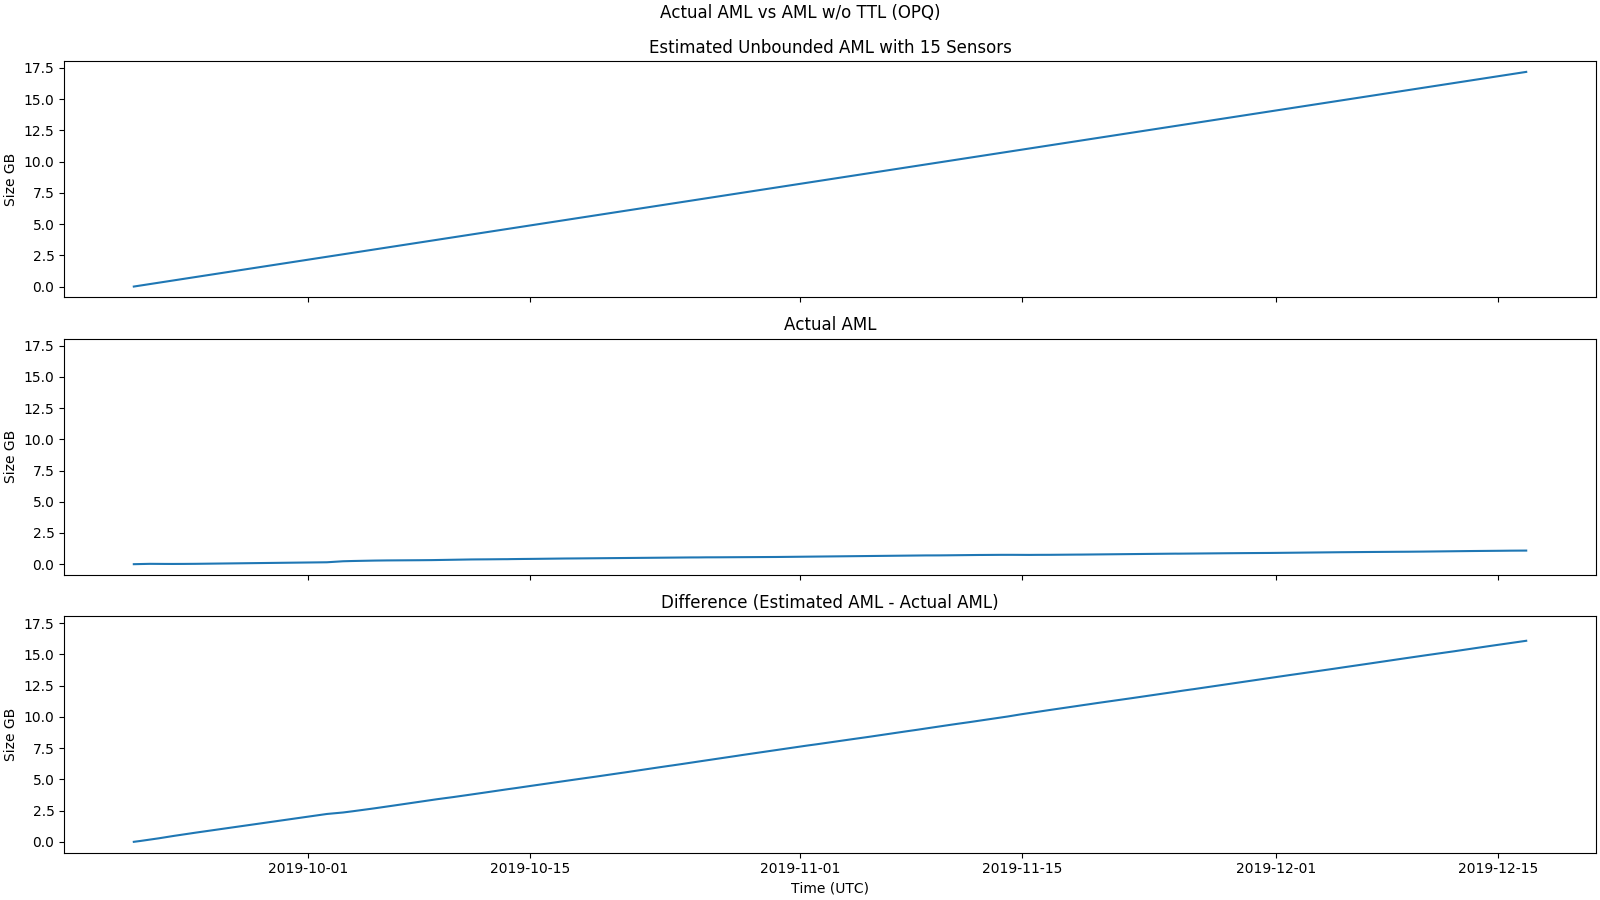
\includegraphics[width=\linewidth]{figures/actual_aml_vs_unbounded_opq.png}
    \caption{Actual AML vs Unbounded AML for OPQ}
    \label{fig:actual_aml_vs_unbounded_opq}
\end{figure}

This data was not affected by the implicit TTL parameter and portrays accurate unbounded versus bounded growth. We can see that over the same time period, AML with TTL saved us about 17.5 GB worth of data versus a store everything approach.

\paragraph{DL Versus Estimated Growth}
Figure~\ref{fig:actual_dl_vs_unbounded_opq} shows the actual DL vs unbounded DL. The Detection Level contains metadata and data bounded by a window which may or may not include signals of interest.

\begin{figure}[H]
    \centering
    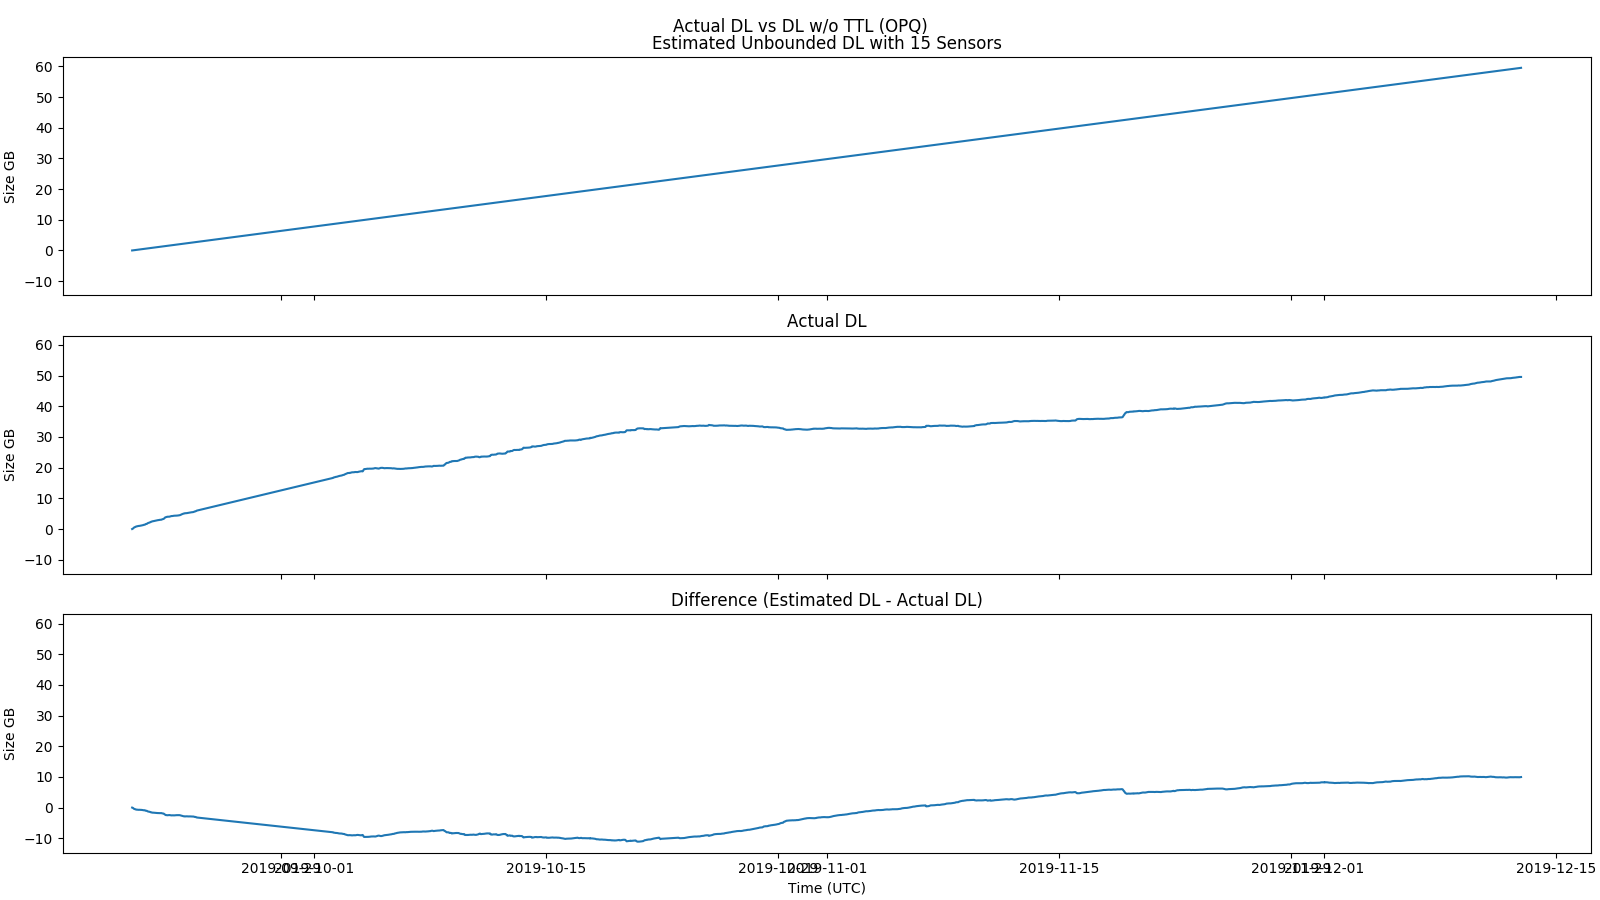
\includegraphics[width=\linewidth]{figures/actual_dl_vs_unbounded_opq.png}
    \caption{Actual DL vs Unbounded DL for OPQ}
    \label{fig:actual_dl_vs_unbounded_opq}
\end{figure}

This data was affected by the implicit TTL parameter and does not portray accurate unbounded versus bounded growth. Instead, the implicit TTL parameter models are actual growth pretty closely and the actual data is about 20 GB larger than the estimated data growth.

\paragraph{IL Versus Estimated Growth}
Figure~\ref{fig:actual_il_vs_unbounded_opq} shows the actual IL vs unbounded IL. The Incident Level contains metadata and data over window that contains classified signals of interest.

\begin{figure}[H]
    \centering
    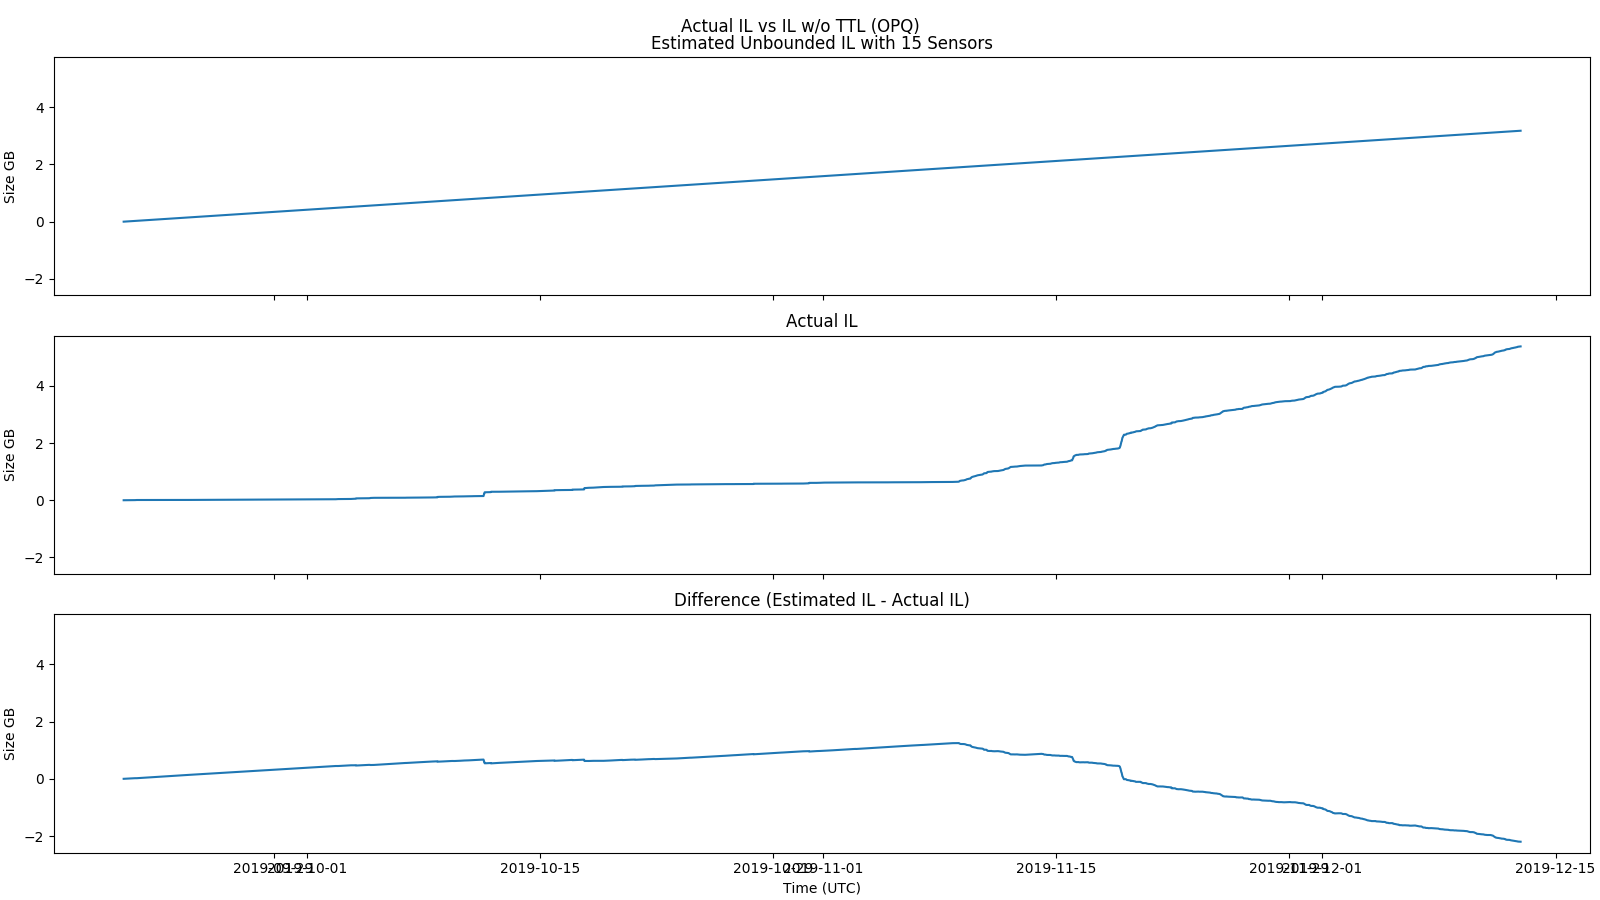
\includegraphics[width=\linewidth]{figures/actual_il_vs_unbounded_opq.png}
    \caption{Actual IL vs Unbounded IL for OPQ}
    \label{fig:actual_il_vs_unbounded_opq}
\end{figure}

This data was affected by the implicit TTL parameter and does not portray accurate unbounded versus bounded growth. Instead, we can see that the actual size of the IL tracks pretty closely to the estimated maximum bounds. At the end of the data collection period, OPQ collected about 4GB less worth of data than what was estimated.

\paragraph{PL Versus Estimated Growth}
Figure shows the actual PL vs unbounded PL.

% TODO
TODO

\paragraph{Laha Versus Estimated Growth}
Finally, I examine the total size of Laha and compare it to the estimated bounds of Laha without TTL. This takes into account all levels within the Laha hierarchy.

Figure~\ref{fig:actual_laha_vs_unbounded_opq} compares the actual bounds of the entire network to the estimated bounds.

\begin{figure}[H]
    \centering
    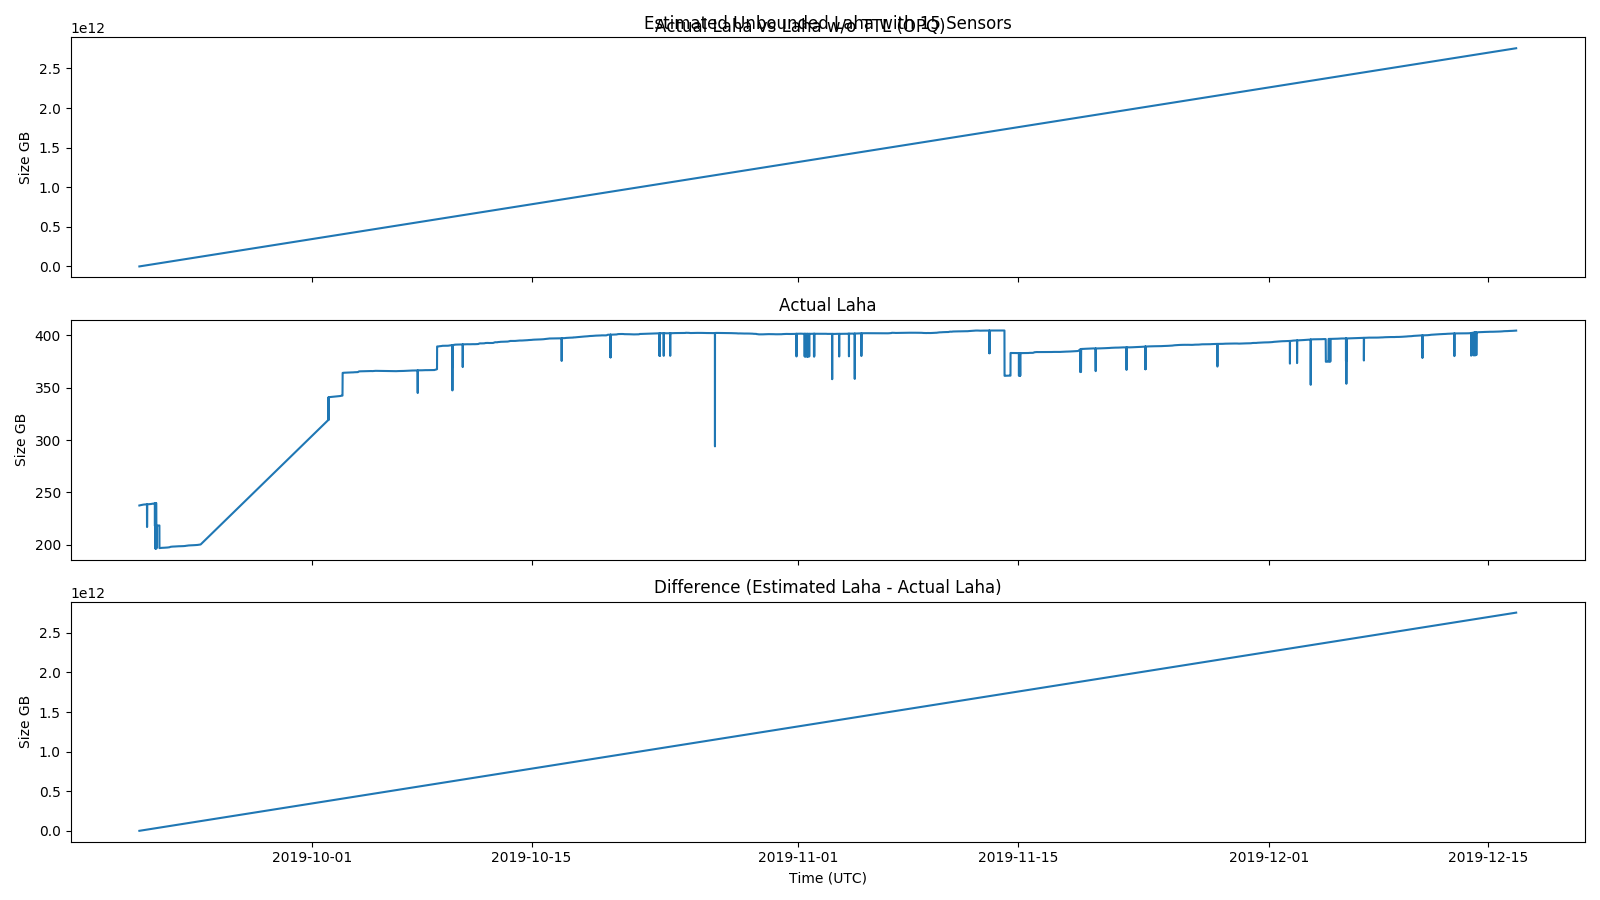
\includegraphics[width=\linewidth]{figures/actual_laha_vs_unbounded_opq.png}
    \caption{Actual Laha vs Unbounded Laha for OPQ}
    \label{fig:actual_laha_vs_unbounded_opq}
\end{figure}

This result is a little unsatisfying. The data growth of the IML is pretty much the only feature evident in this plot. To better understand the growth of the entire system, I removed the IML as shown in Figure~\ref{fig:actual_laha_vs_unbounded_no_iml_opq}.

\begin{figure}[H]
    \centering
    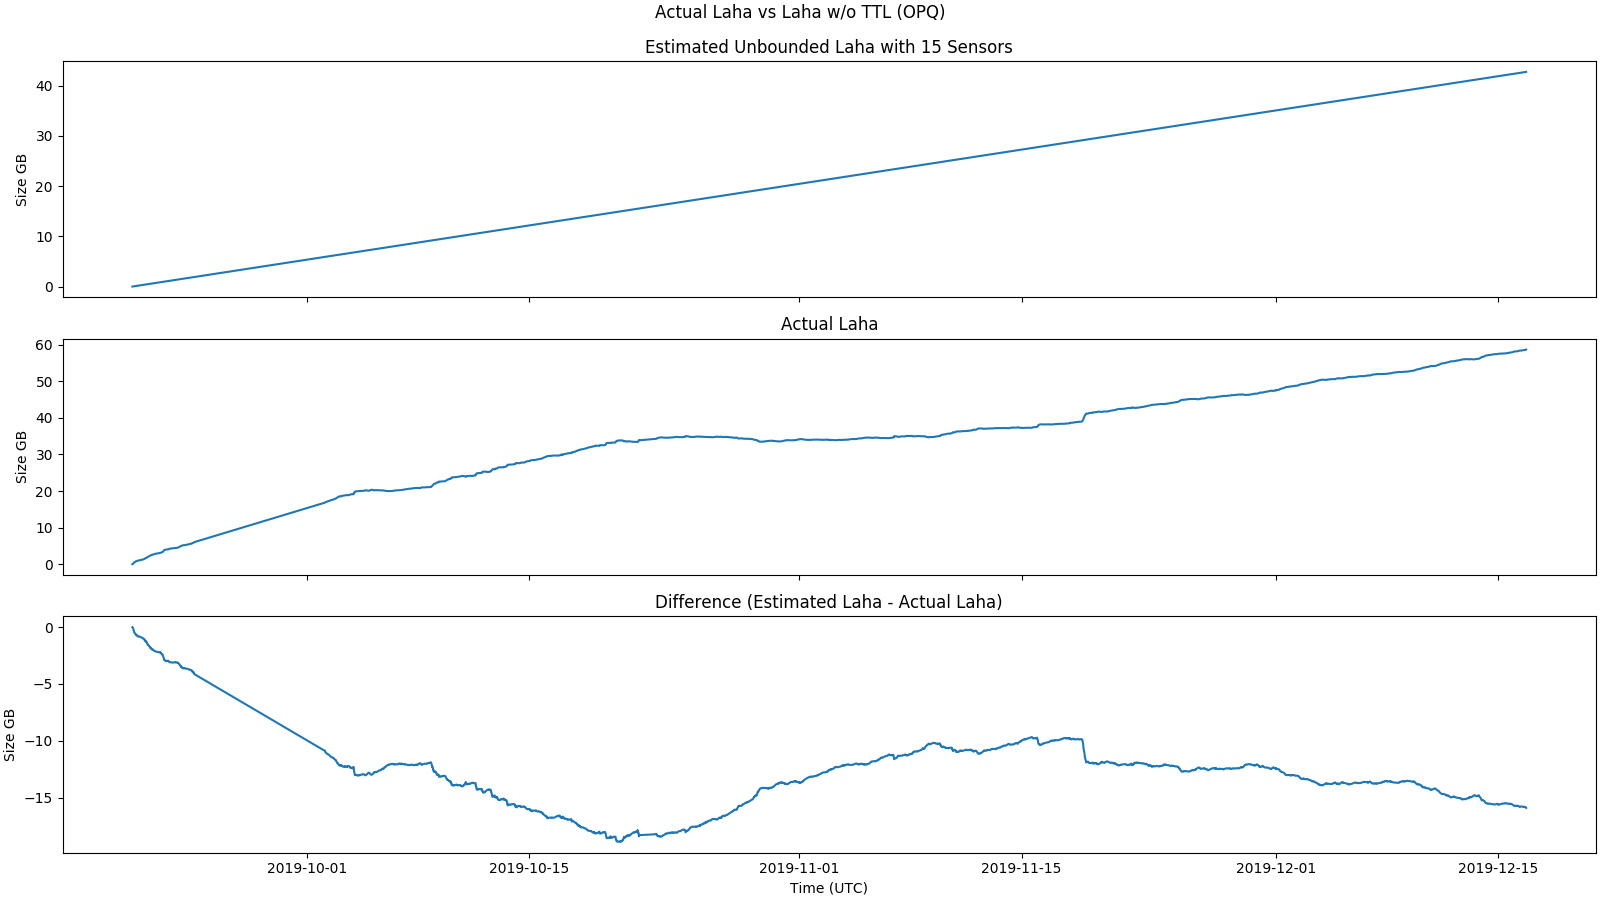
\includegraphics[width=\linewidth]{figures/actual_laha_vs_unbounded_opq_no_iml.png}
    \caption{Actual Laha vs Unbounded Laha for OPQ (No IML)}
    \label{fig:actual_laha_vs_unbounded_no_iml_opq}
\end{figure}

Over a time period of 2 and a half months, the OPQ network saved about 20GB of data as compared to a store everything approach (not including the IML which saved about 2.5 TB of data). Of course, I would expect this difference to be greater if I had actual metrics for the DL, IL and PL that did not have a built-in implicit TTL parameter. Even with the built-in parameter, the savings gained from the AML alone is significant.

\subsubsection{DSN System Requirements OPQ: Comparing Results to Simulated Data}

Next I will compare the results gathered from the OPQ deployment to the simulated bounds found in Section~\ref{sssec:evaluation_of_ttl}.

Similar to the previous comparisons, I will offset the actual data to ``force" the data to start from zero.

The simulated data had to be aligned with the collected metrics to perform this evaluation. The alignment works by binning all relevant timestamps to the nearest minute between the two data series.

\paragraph{IML Versus Simulated Growth}
The Instantaneous Measurements Level (IML) contains raw samples from sensors. Figure~\ref{fig:actual_iml_vs_sim_opq} shows the actual IML vs estimated IML.

\begin{figure}[H]
    \centering
    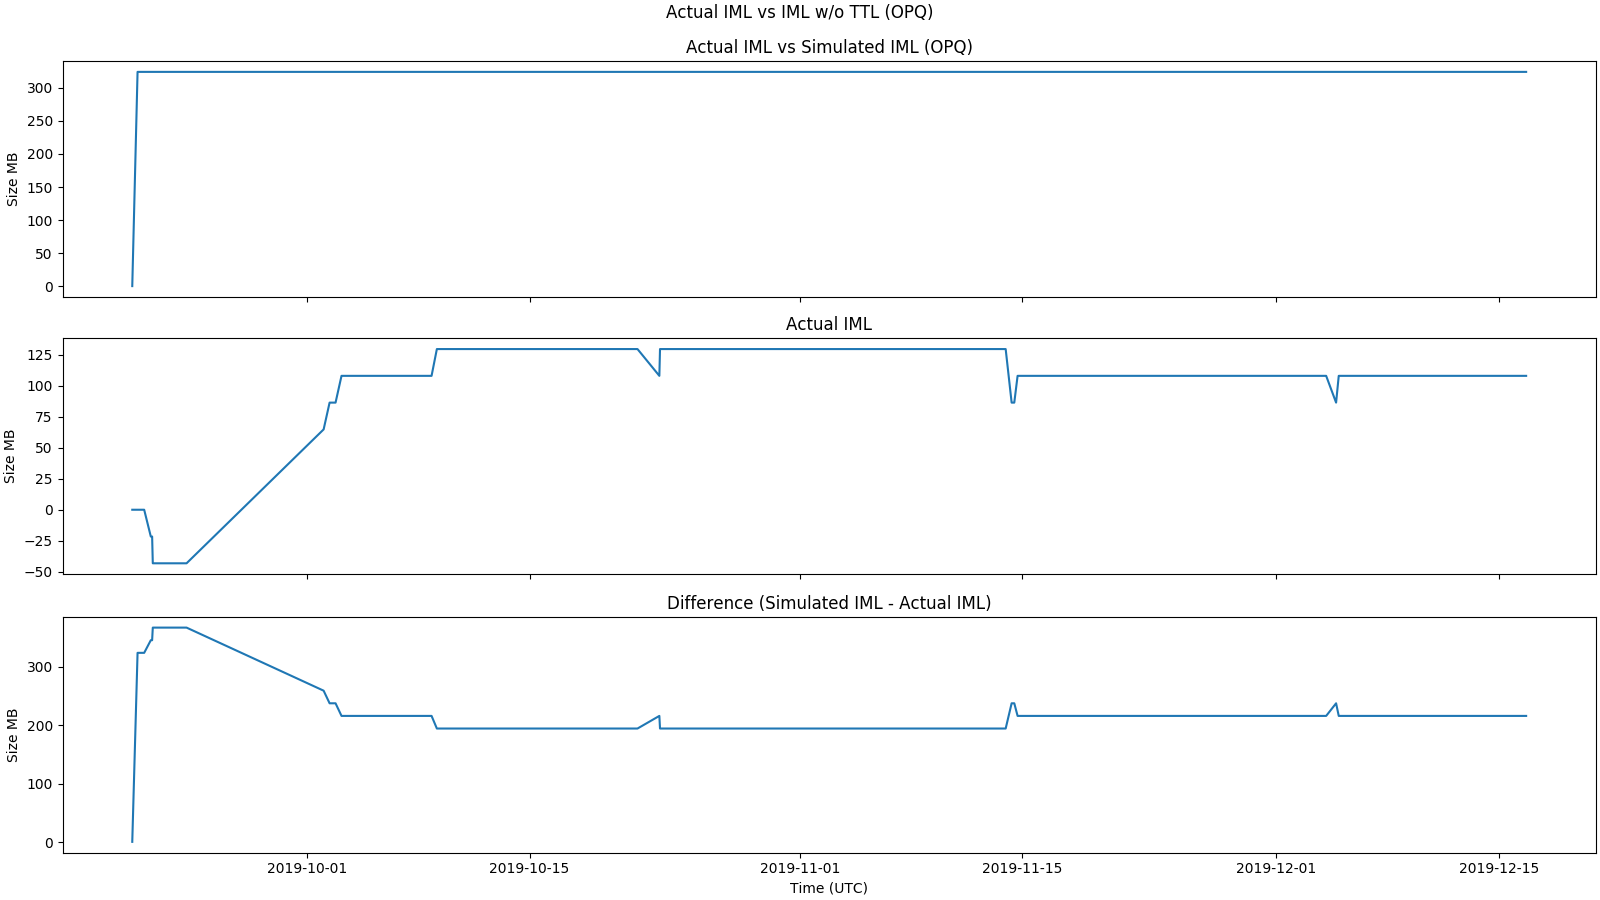
\includegraphics[width=\linewidth]{figures/actual_iml_vs_sim_opq.png}
    \caption{Actual IML vs Simulation IML for OPQ}
    \label{fig:actual_iml_vs_sim_opq}
\end{figure}

The simulation tracks the actual data pretty closely with a difference hovering around 0 MB. The simulation assumes that 15 sensors are always sending, whereas the actual data fluctuates with the number of active sensors.

\paragraph{AML Versus Simulated Growth}
The Aggregate Measurements Level (AML) contains rolled up summary statistics of selected features generated from IML data. Figure~\ref{fig:actual_aml_vs_sim_opq} shows the actual AML vs estimated AML.

\begin{figure}[H]
    \centering
    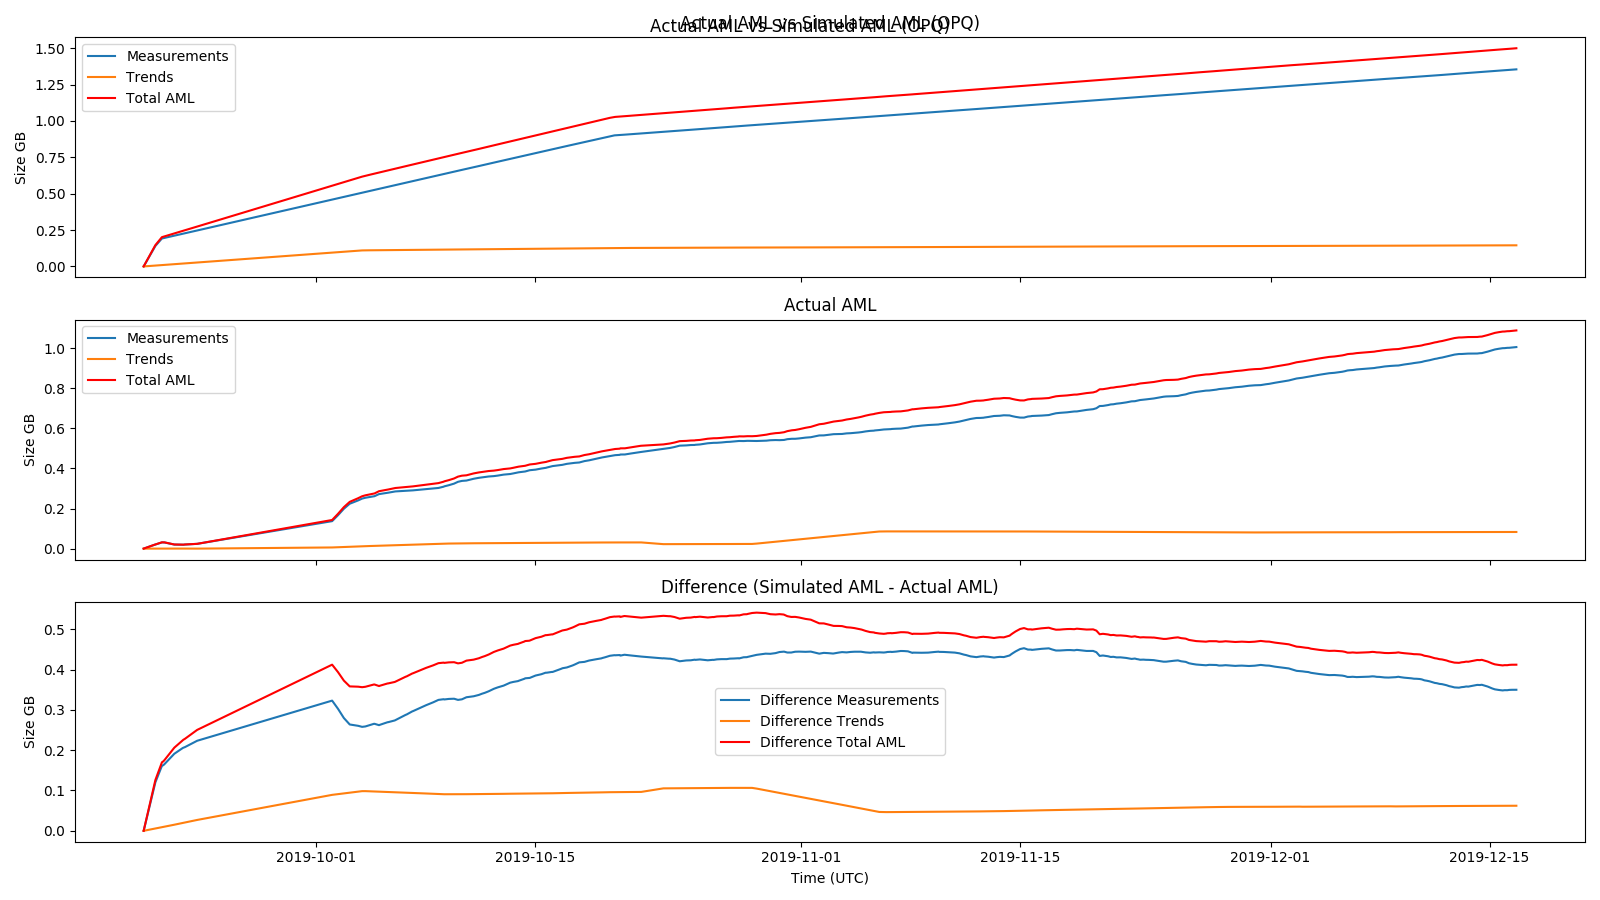
\includegraphics[width=\linewidth]{figures/actual_aml_vs_sim_opq.png}
    \caption{Actual AML vs Simulation AML for OPQ}
    \label{fig:actual_aml_vs_sim_opq}
\end{figure}

The simulated AML data trends closely with the actual data. There is a slight underestimation early on, but converges to close to 0 GB by the end of the data collection.

\paragraph{DL Versus Simulated Growth}
The Detection Level (DL) contains metadata and a window of raw data that may or may not include signals of interest. Figure~\ref{fig:actual_dl_vs_sim_opq} shows the actual DL vs estimated DL.

\begin{figure}[H]
    \centering
    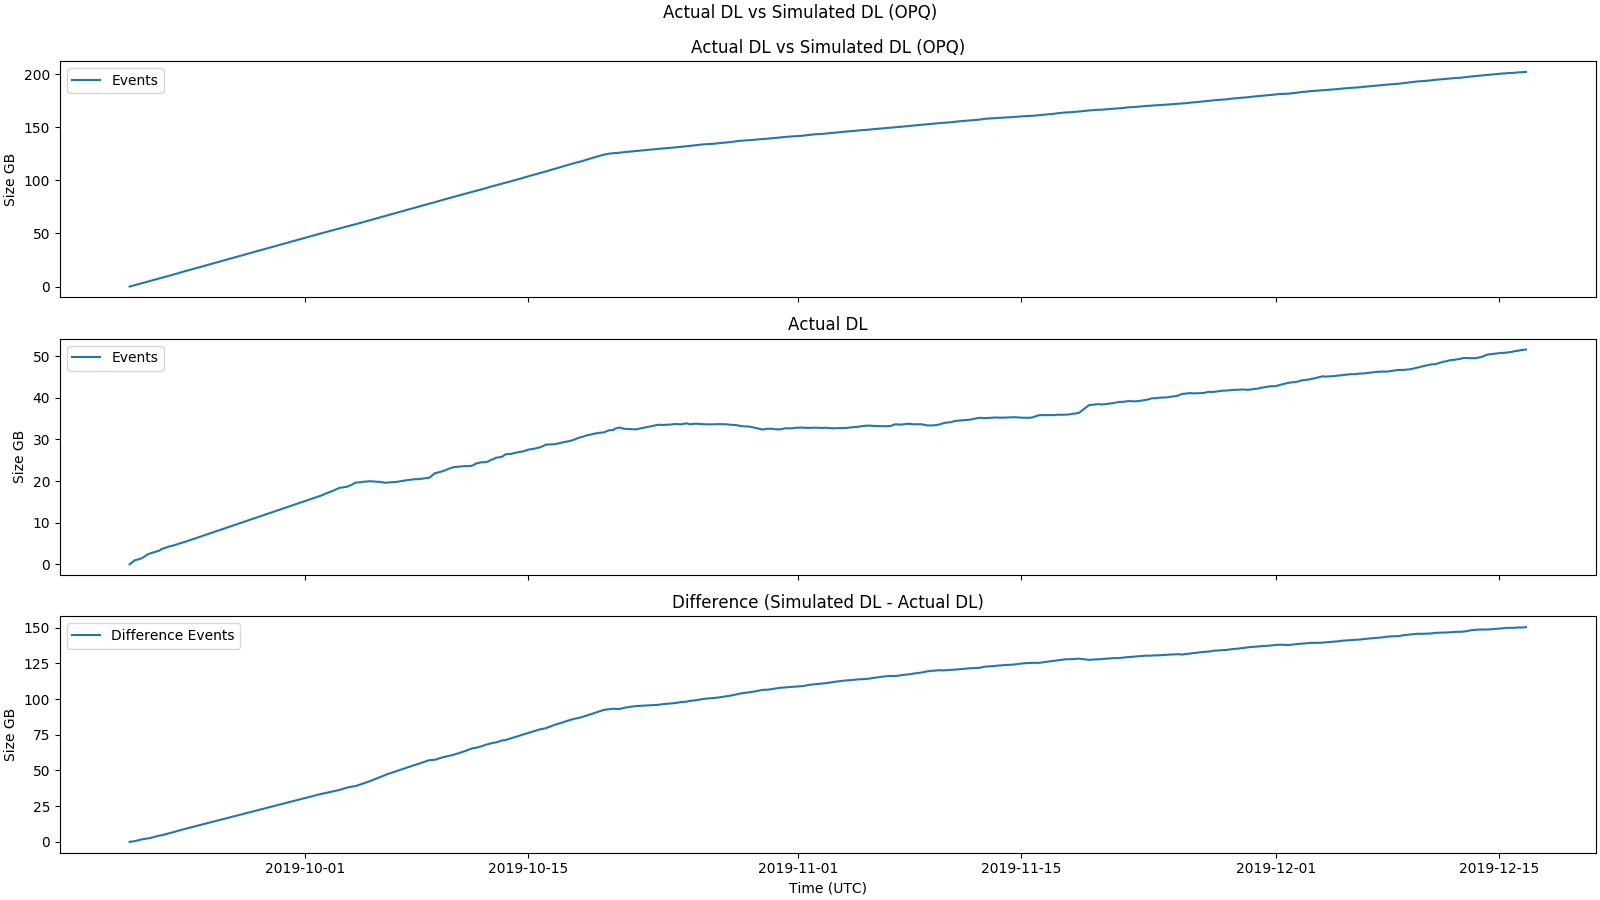
\includegraphics[width=\linewidth]{figures/actual_dl_vs_sim_opq.png}
    \caption{Actual DL vs Simulation DL for OPQ}
    \label{fig:actual_dl_vs_sim_opq}
\end{figure}

Although the simulated data has a similar shape to the actual data for the DL, there is a large offset between the simulation and the actual data. There are several reasons for this offset. The parameters passed into the simulation have somewhat large variances. The leading issue though, is that the simulation assumes that each device produces the same amount of Detections. In practice, certain boxes produce many Detections while others produce relatively few Detections. These differences can likely be attributed to the offset. On the bright side, at least the actual data is less than the simulated data and not the other way around!

OPQ saves near 150 GB of data as compared to the simulation.

\paragraph{IL Versus Simulated Growth}
The Incidents Level (IL) contains metadata and a window of data that contains classified signals of interest. Figure~\ref{fig:actual_il_vs_sim_opq} shows the actual IL vs estimated IL.

\begin{figure}[H]
    \centering
    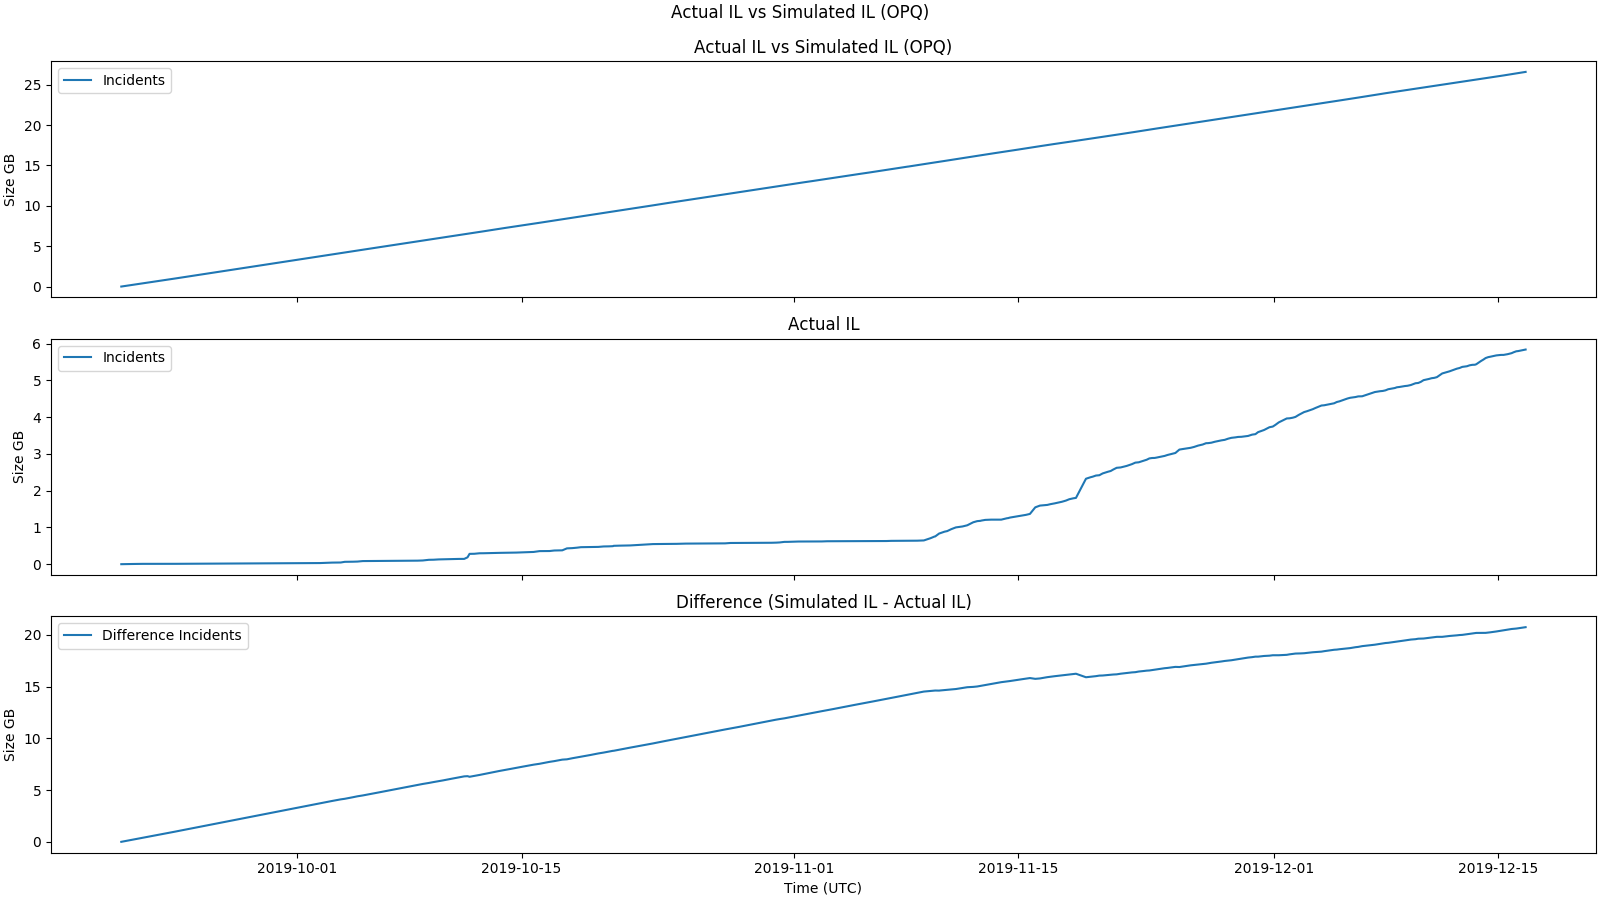
\includegraphics[width=\linewidth]{figures/actual_il_vs_sim_opq.png}
    \caption{Actual IL vs Simulation IL for OPQ}
    \label{fig:actual_il_vs_sim_opq}
\end{figure}

The simulated IL data is better than the simulated DL data, but still displays an offset, likely for the same reasons as the DL. OPQ saves 20 GB in the IL compared to the simulated IL.

\paragraph{PL Versus Simulated Growth}
Figure shows the actual PL vs estimated PL.

% TODO
TODO

\paragraph{Laha Versus Simulated Growth}
Figure~\ref{fig:actual_laha_vs_sim_opq} shows the actual Laha vs estimated Laha.

The large offsets in the simulated DL and IL data create the overall trends in this plot. The shapes of the trends are similar but the offset shows that OPQ saves near 150 GB of data over the same time period as the simulation.

\begin{figure}[H]
    \centering
    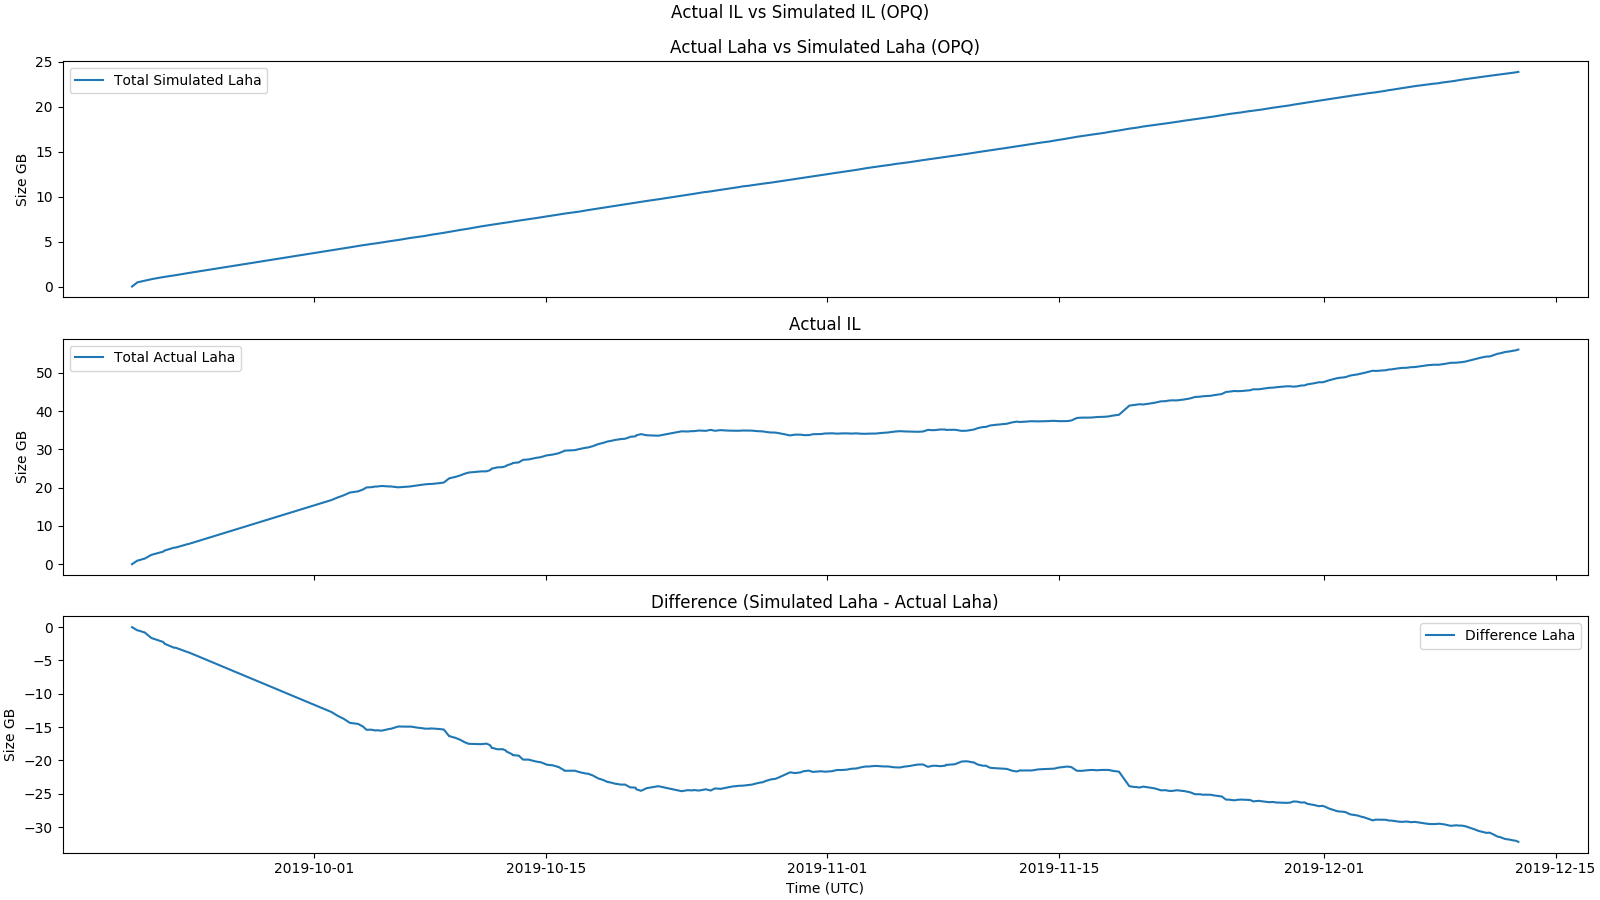
\includegraphics[width=\linewidth]{figures/actual_laha_vs_sim_opq.png}
    \caption{Actual Laha vs Simulation Laha for OPQ}
    \label{fig:actual_laha_vs_sim_opq}
\end{figure}

\paragraph{Discussion on Estimation Versus Simulation}

I compared actual data for each level in the Laha hierarchy to both estimated bounds and simulated bounds. Both approaches show promising results for certain levels. The estimated bounds are better suited for examining the DL, IL, and PL whereas the simulated bounds are better for examining the IML and AML. The estimated bounds include an implicit TTL parameter where the simulated bounds actually performs TTL in the simulation.

Future work should look at expanding the collection of parameters saved when items are garbage collected. This would allow better estimated bounds without TTL and provide better parameters to the simulation.

Both approaches showed significant data savings when utilizing the data management techniques within Laha.

\subsubsection{DSN System Requirements OPQ: CPU, Memory, and Disk Utilization}

We collected CPU, memory, and disk utilization during the deployment of the OPQ network. It would be prudent to first discuss the details of the system that the OPQ network is running on.

Makai, Mauka, View, MongoDB, and Health are all running on the same virtual server hosted by the University's Information Technology Services. The server is running Red Hat Enterprise Linux Server release 7.7 (Maipo). Due to a configuration error, the server only ran with a single virtual CPU up until October 28, 2019. After that time period, a second virtual CPU was added. Each virtual CPU is an Intel Xeon E5-2687W v3 running at 3.10 GHz. The system has 8 GB of main memory and 8 GB of swap space. The system has 1 TB of hard disk storage.

These system statistics are for the entire virtual server and include loads of all virtualized OPQ services. Mauka is certainly doing the most work of any of the virtualized services, but it should be noted that these statistics also include overhead incurred from other OPQ and OS services.

It should be noted that I attempted to collect the same statistics from the Lokahi network, but due to system requirements and a complicated distributed architecture, we were not able to collect metrics for the entire system. For example, many of Lokahi's services use specialized Amazon Web Services (AWS) services which do not expose similar metrics that are exposed by OPQ. For that reason, we will only examine the OPQ network in detail.

Figure~\ref{fig:actual_system_opq} shows the OPQ system resource utilization over a period of two and a half months.

\begin{figure}[H]
    \centering
    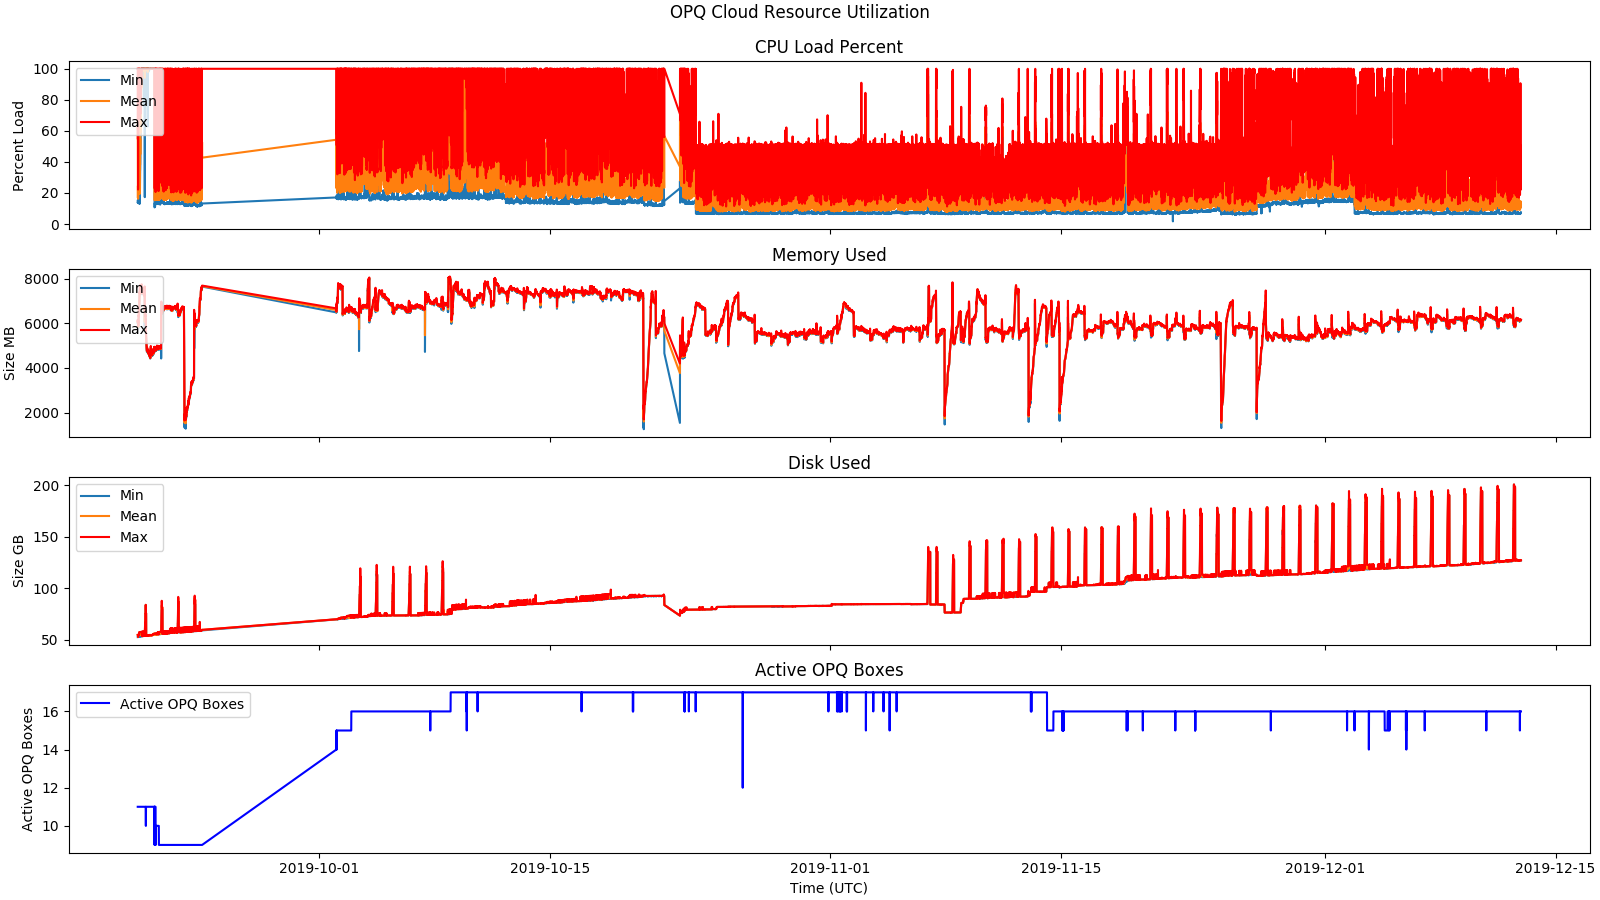
\includegraphics[width=\linewidth]{figures/actual_system_opq.png}
    \caption{System Utilization for OPQ}
    \label{fig:actual_system_opq}
\end{figure}

You'll note a gaps in the data in early and mid October. These were caused by a mix-up in deployed branches where one of the branches did not have collected of system statistics enabled.

The top panel shows the minimum, mean, and maximum CPU load. Each triplet of min, mean, and max values are aggregated over 30 sample points. So even though the CPU hits 100\% utilization quite often, the mean of the CPU utilization is much lower, rarely rising over 40\%. A slight decrease (~5\%) in CPU load can be observed when the second virtual CPU was added to the system.

I expect that we could double the amount of deployed sensors to 30 and still see mean CPU utilization less than 80\%. Beyond that would require either more powerful hardware or distributing OPQ services over multiple servers.

The second panel shows memory utilization. OPQ utilizes on average close to 75\% of the available memory. I dug a little bit deeper into how the memory was being utilized and found a perhaps unsurprising result. Table~\ref{table:mem_utilization} shows the breakdown of largest memory utilization on our system.

\begin{table}[H]
    \centering
    \caption{OPQ Large Memory Utilization}
    \begin{tabularx}{\textwidth}{Xl}
        \toprule
        \textbf{Process} & \textbf{\% Memory} \\
        \midrule
        MongoDB & 51 \\
        OPQ Mauka & 8 \\
        OPQ View & .8 \\
        OPQ Makai & .3 \\
        Docker & .3 \\
        OPQ Box Updater & .1 \\
        JournalD & .1 \\
        \bottomrule
    \end{tabularx}
    \label{table:mem_utilization}
\end{table}

MongoDB uses over half of our available memory! This should be somewhat unsurprising because MongoDB aggressively caches data in-memory for efficient queries. No matter how much memory is on our system, MongoDB will use a large chunk of it. All of the OPQ Mauka processes combined only add up to about 8\% memory utilization with 15 sensors. I estimate that on current hardware, Mauka could handle up to about 100 sensors and still remain within 80\% memory utilization (of course this would have an adverse affect on MongoDB caching).

The third panel shows disk usage over time. As of about two and a half months into data collection, the server is storing about 130 GB worth of data. One interesting feature of this plot are the periodic spikes. The periodic spikes are caused by daily database backups. Every day, a backup of the database is performed, compressed, and written to disk. It is then uploaded to cloud storage and on successful upload, deleted locally. There is a large gap of these spike near the end of October and beginning of November. This gap is the result of a Docker bug that inhibited our system from performing daily backups. I changed the backup routine to use a local MongoDB client rather than one provided by Docker and the daily backups resumed.

The bottom panel shows the number of active OPQ Boxes sending over time. There does not appear to be a large correlation between the number of boxes sending and system resource utilization. This is likely due to the fact that the standard deviation between the number of active OPQ Boxes is quite small ($\sigma=1.63$).

\subsection{DSN System Requirements: Lokahi}\label{subsec:dsn-system-requirements:-lokahi}

\subsubsection{DSN System Requirements Lokahi: IML}

\subsubsection{DSN System Requirements Lokahi: AML}

\subsubsection{DSN System Requirements Lokahi: DL}

\subsubsection{DSN System Requirements Lokahi: IL}

\subsubsection{DSN System Requirements Lokahi: PL}
